\documentclass[english, a4paper,11pt]{article}
\usepackage[latin1]{inputenc}
\usepackage[T1]{fontenc}
\usepackage{bbm}
\usepackage{amsmath}
\usepackage{indentfirst}
\usepackage{fullpage}
\usepackage{url}
\usepackage{graphicx}
\usepackage{geometry}
\geometry{verbose,tmargin=3cm,bmargin=2cm,lmargin=2cm,rmargin=2cm}
\usepackage{babel}
\usepackage[center,footnotesize]{caption}
\usepackage[section]{placeins}
\usepackage{subfig}

\title{Solutions - Series 4}
\date{October 11, 2011}
\author{Genomics and bioinformatics - Week 4}

\begin{document}
\maketitle

\section{Sequence alignment}

\emph{Match:}  \texttt{+1}, \emph{Mismatch:} \texttt{-1}, \emph{Gap:} \texttt{0}

Sequence 1: \texttt{GAATTCAGA}

Sequence 2: \texttt{GGATCGA}.\\

Step 1: INITIALIZATION

Create a matrix with \texttt{m + 1} columns and \texttt{n + 1} rows where \texttt{m} and \texttt{n} correspond to the sizes of Sequences 1 and 2, respectively. \\


Step 2: SCORING

Using the given scoring scheme, at each cell, 3 scores are calculated:
\begin{itemize}
\item Upper neighbour score + Gap cost
\item Left neighbour score + Gap cost
\item Upper-left neighbour score + Match score (if nucleotides match), \emph{OR} 

Upper-left neighbour score + Mismatch cost (if nucleotides do not match)
\end{itemize}

\indent\emph{The highest score is retained and the arrow is labelled.} The resulting scoring matrix should look something like this, \\

\begin{center}
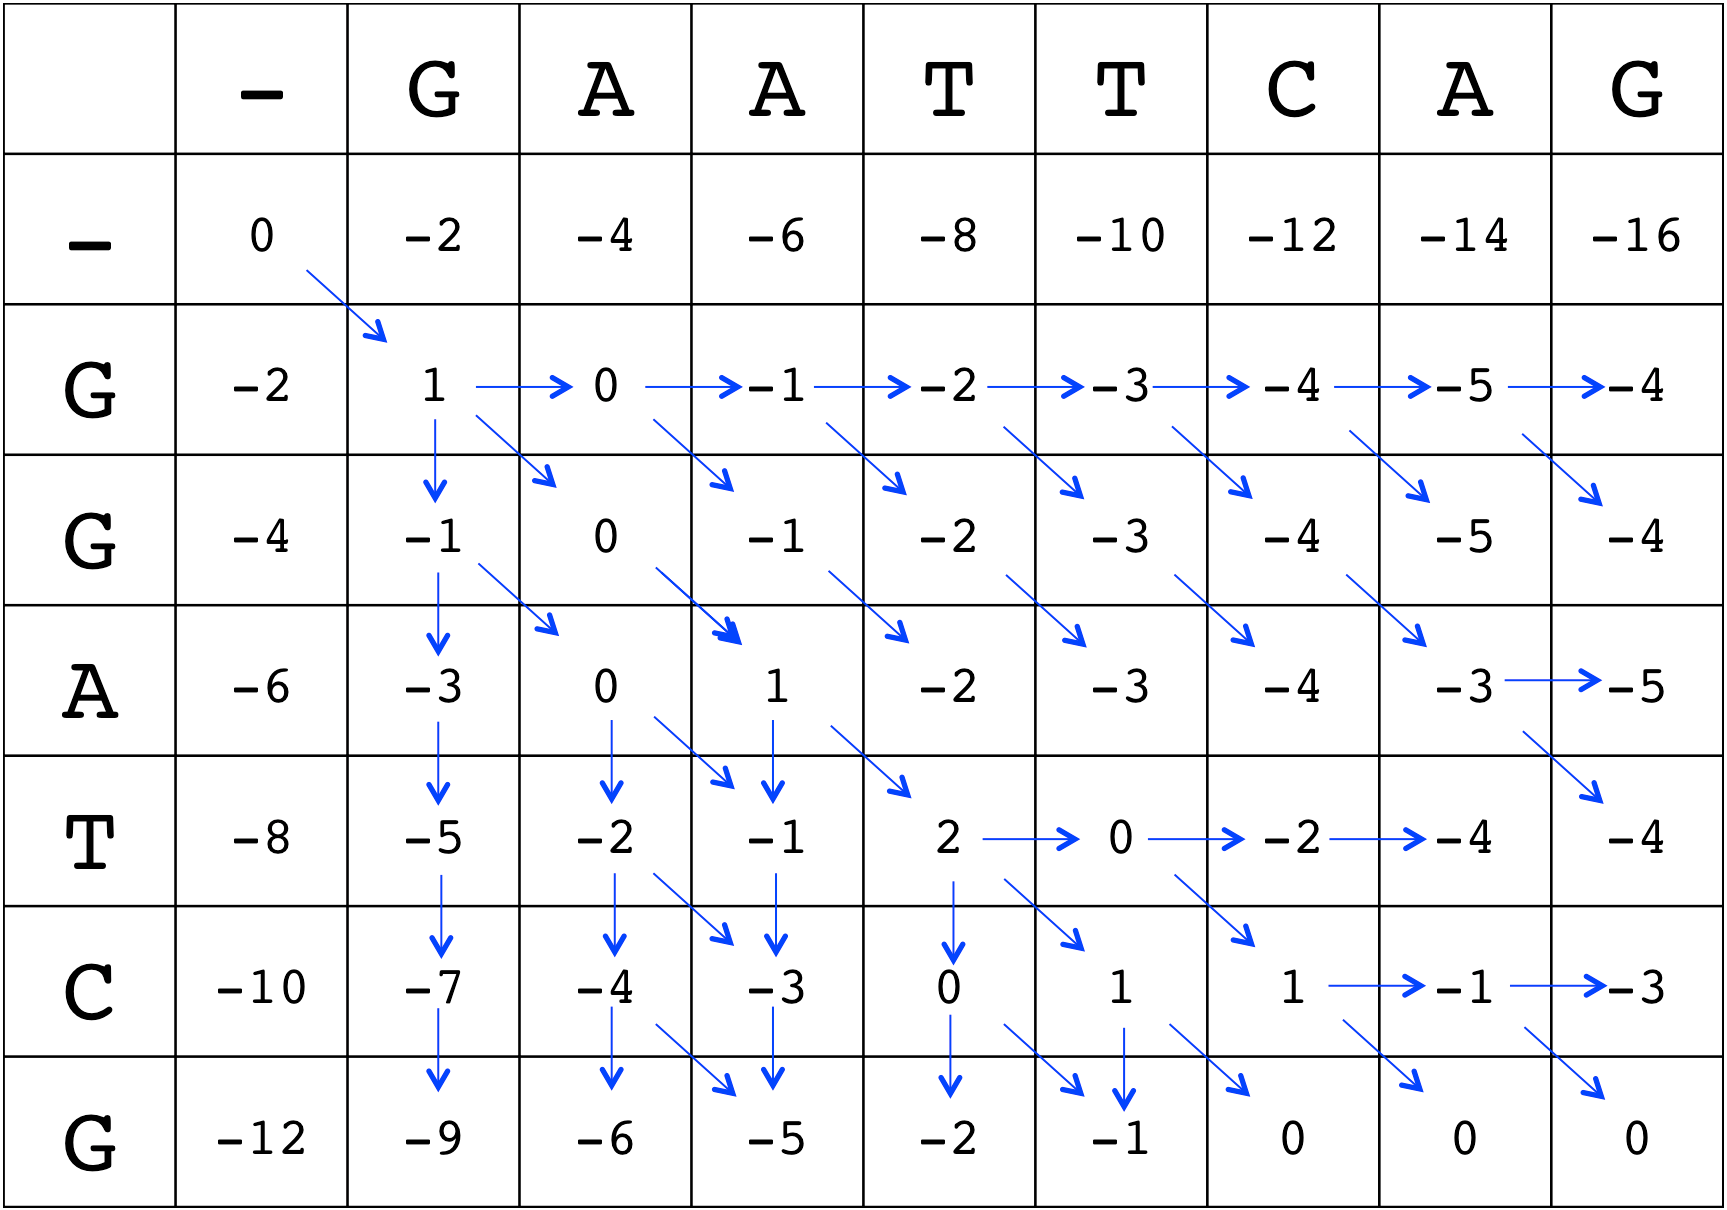
\includegraphics[width=0.6\textwidth]{scoring.png}\\
\end{center}

\pagebreak

Step 3: BACKTRACKING

 The process of deduction of the best alignment from the score matrix is known as traceback. The traceback begins with the last cell to be filled, i.e. the bottom-right cell, and is completed when the first, i.e. the top-left cell of the matrix is reached. Several traceback paths are possible. The solution resulting in the best final score is selected to deduce the optimum alignment. It is possible to have more than one optimum alignment. 

A traceback path for the scoring matrix generated in Step 2 is highlighted below, 

\begin{center}
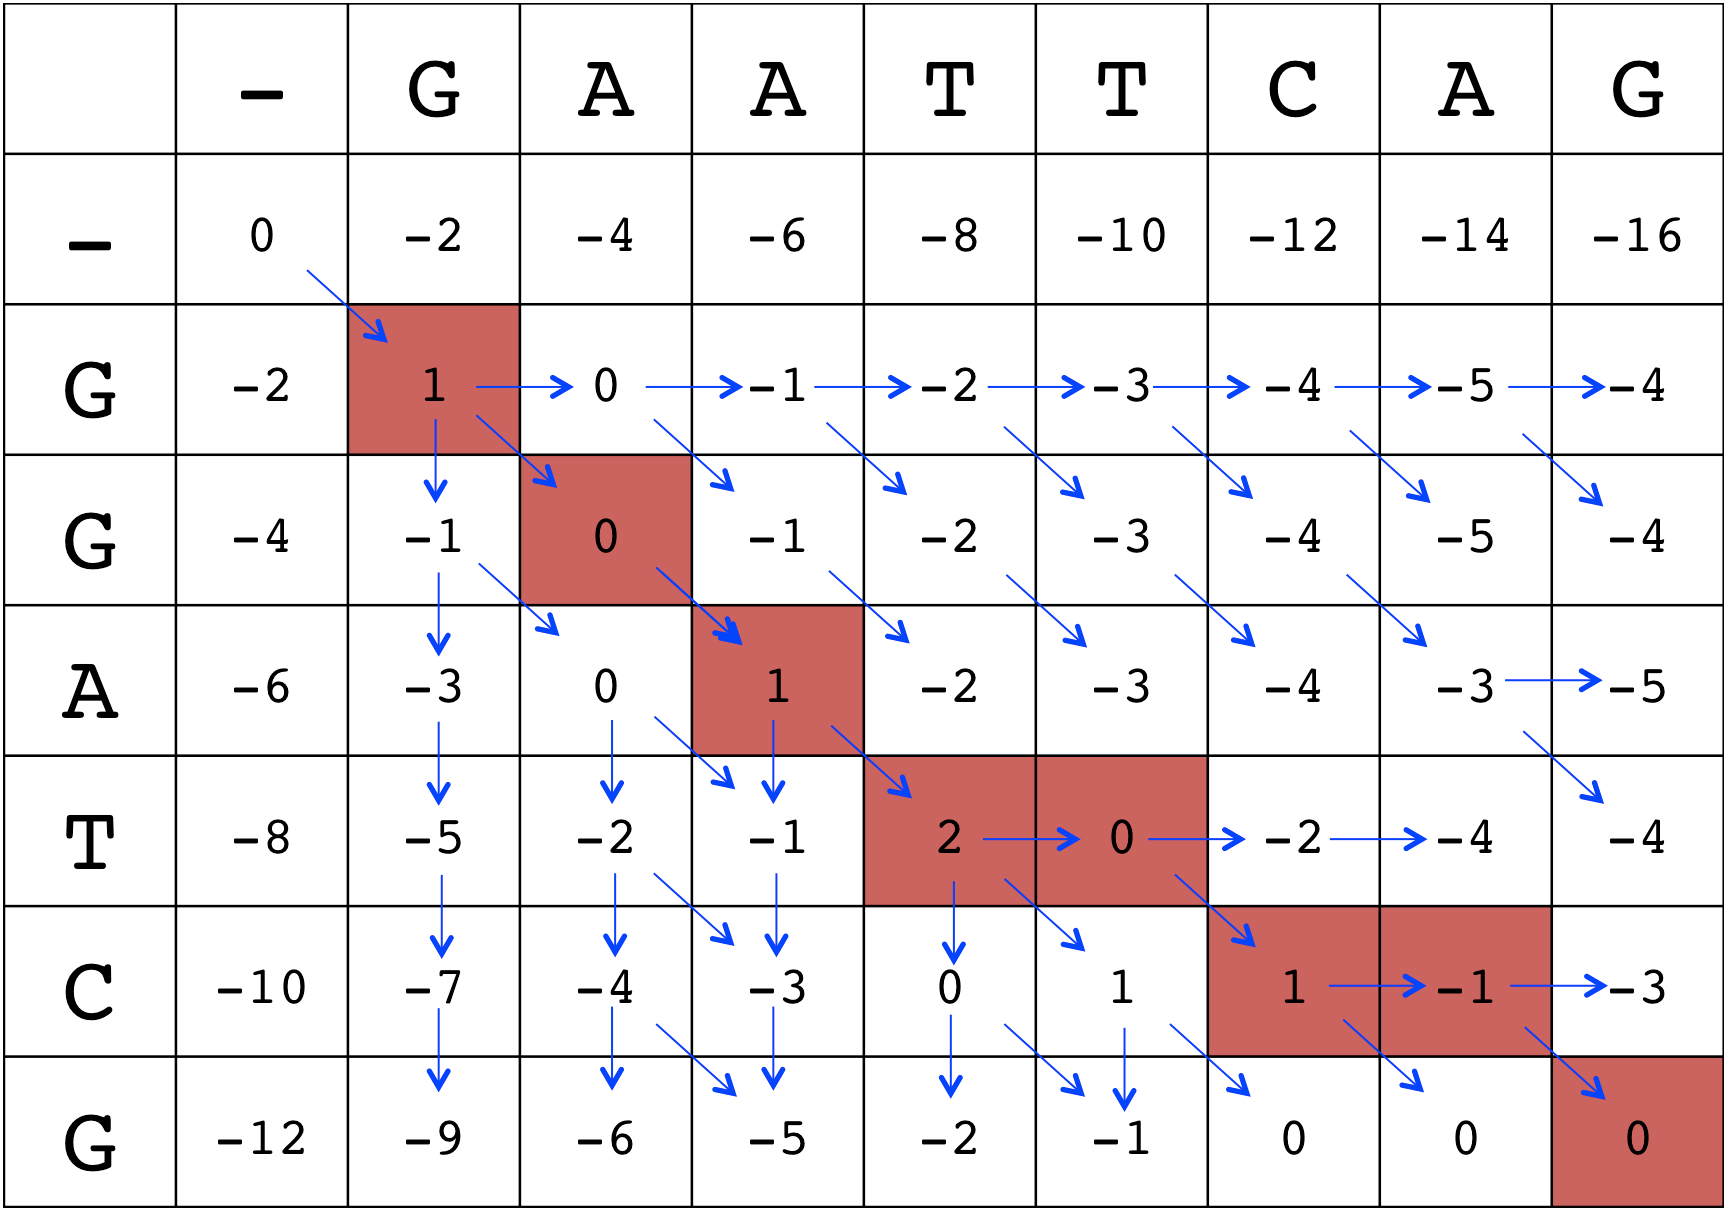
\includegraphics[width=0.6\textwidth]{backtracking.png}
\end{center}

Step 4: ALIGNMENT

After backtracking, the optimal alignment is easy to recover using following the rule,

 \emph{Left} = Gap , \emph{Up} = Insertion, and \emph{Diagonal} = Match 

The optimum alignment for the two sequences \texttt{GAATTCAGA} and \texttt{GGATCGA} is,

\begin{center}
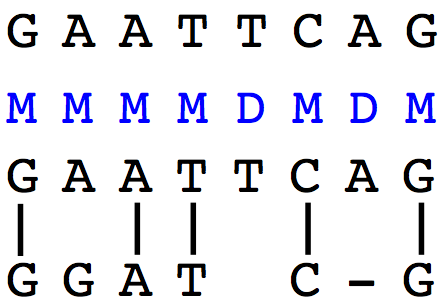
\includegraphics[width=0.2\textwidth]{alignment.png}
\end{center}

\section{Pair HMM}

The corresponding HMM is given by

%
\begin{figure}
\begin{centering}
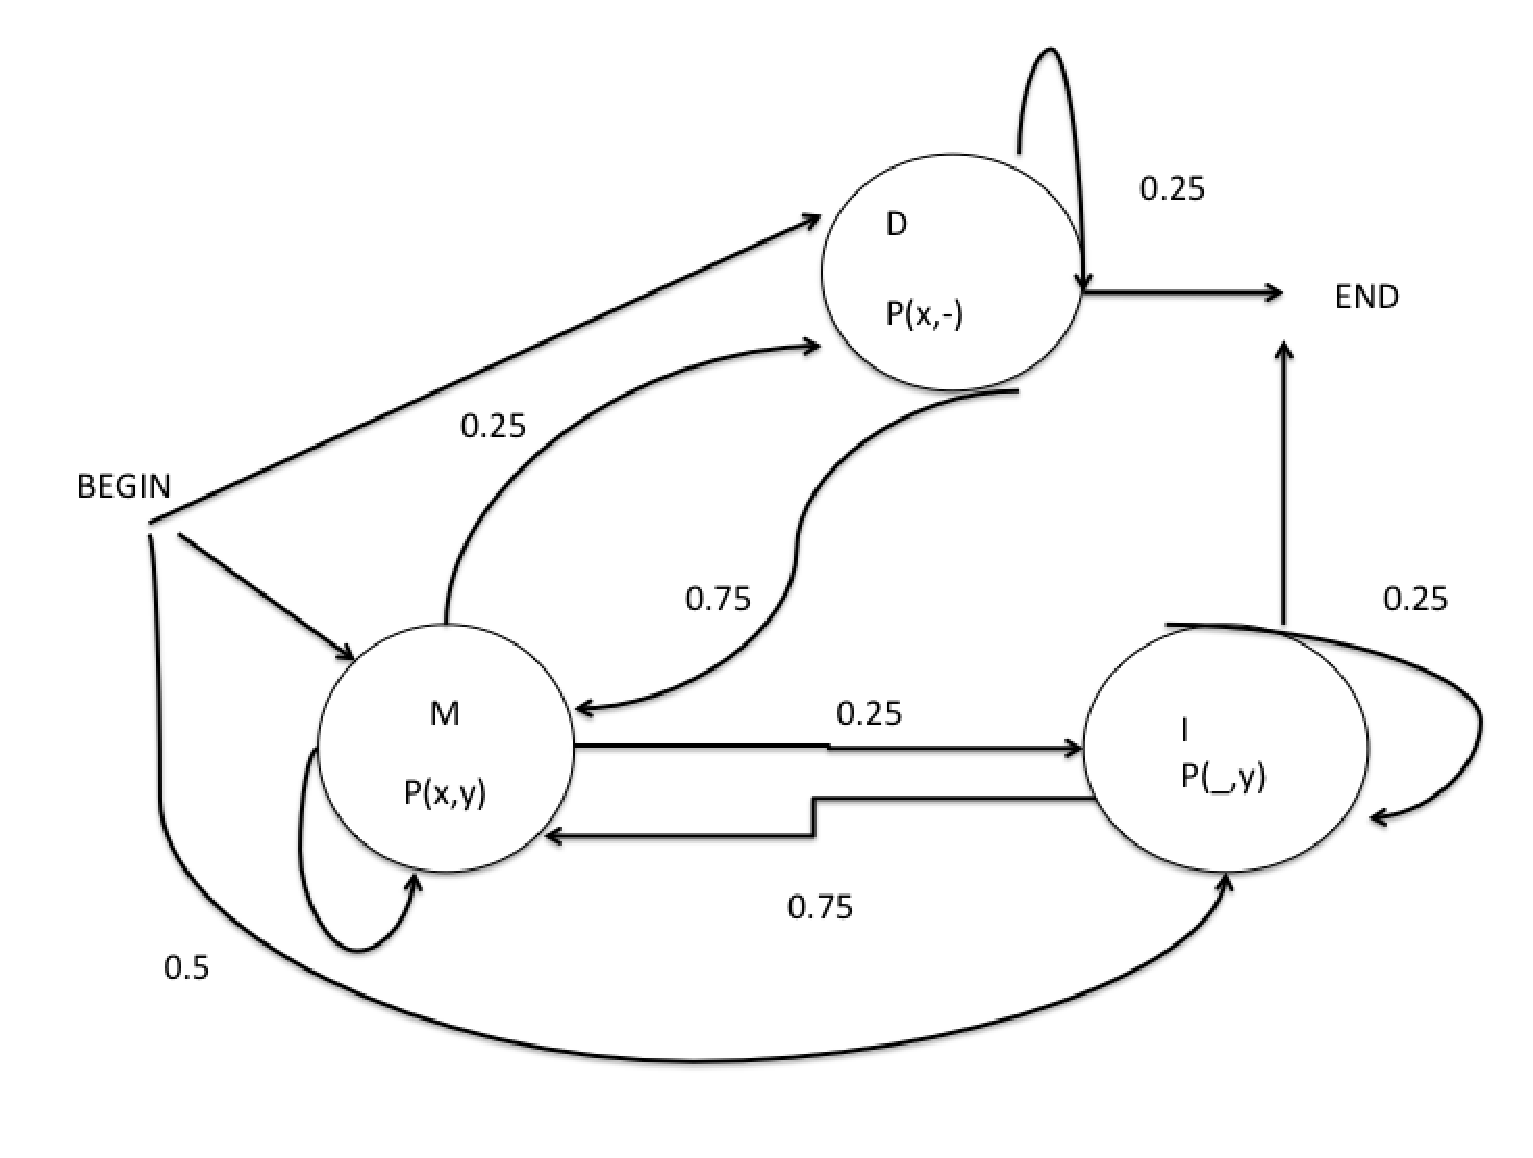
\includegraphics[width=4in]{Slide5}
\par\end{centering}

\caption{The HMM mpdel for sequence alignment}
%
\end{figure}


where, p(x,y)=0.125 and p(x,y)=0.04 for mismatch

p(x,\_)=q(\_,y)=0.25

If we consider all probability values with repesct to a random model
in log-odds

\[
S(x,y)=log\frac{p(x,y)}{p(x)\; p(y)}\]


%
\begin{figure}
\begin{centering}
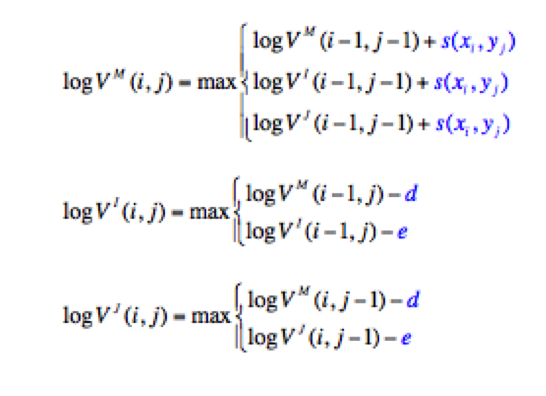
\includegraphics[width=3in]{Viterbi}
\par\end{centering}

\caption{Viterbi Algorithm}
%
\end{figure}
$ $

\[
S(x,y)=1\quad for\quad match\qquad and\quad s(x,y)=-1\quad for\quad mismatch\]


The we can consruct the three matrices for VM, VX and VY by the Viterbi
algorithm

%
\begin{figure}
\begin{centering}
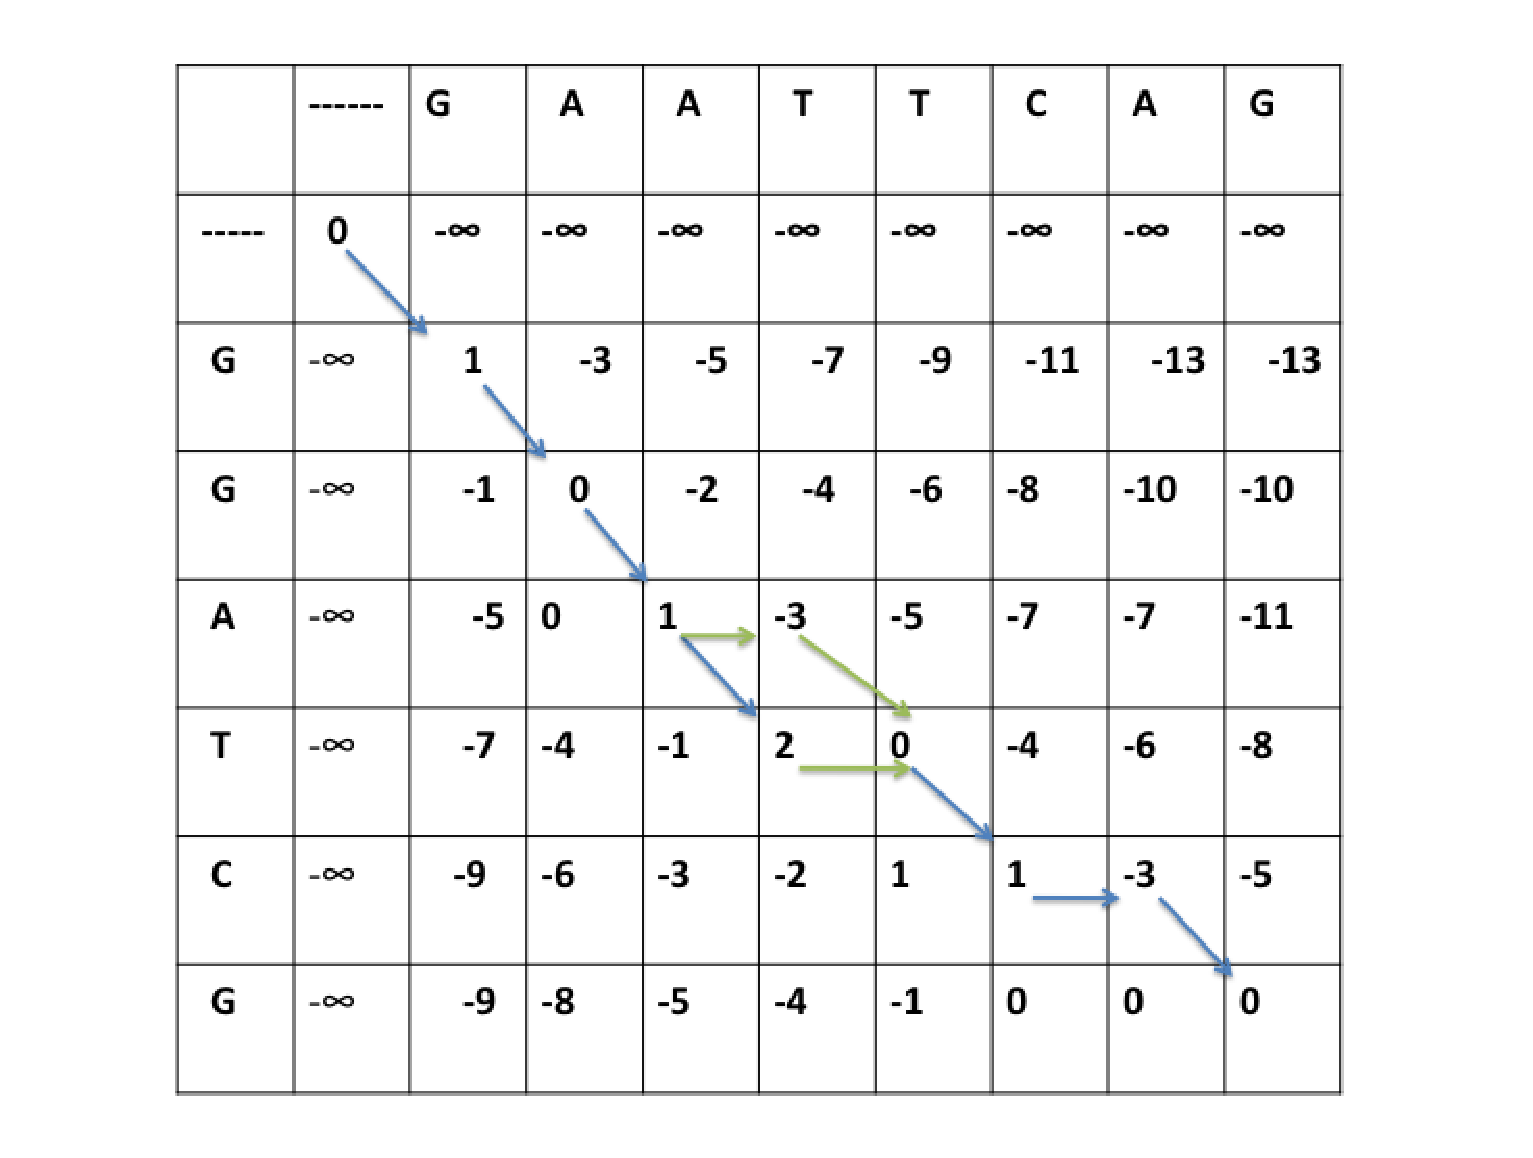
\includegraphics[width=4in]{Slide1}\caption{The matrix for the match state}

\par\end{centering}

%
\end{figure}


%
\begin{figure}
\begin{centering}
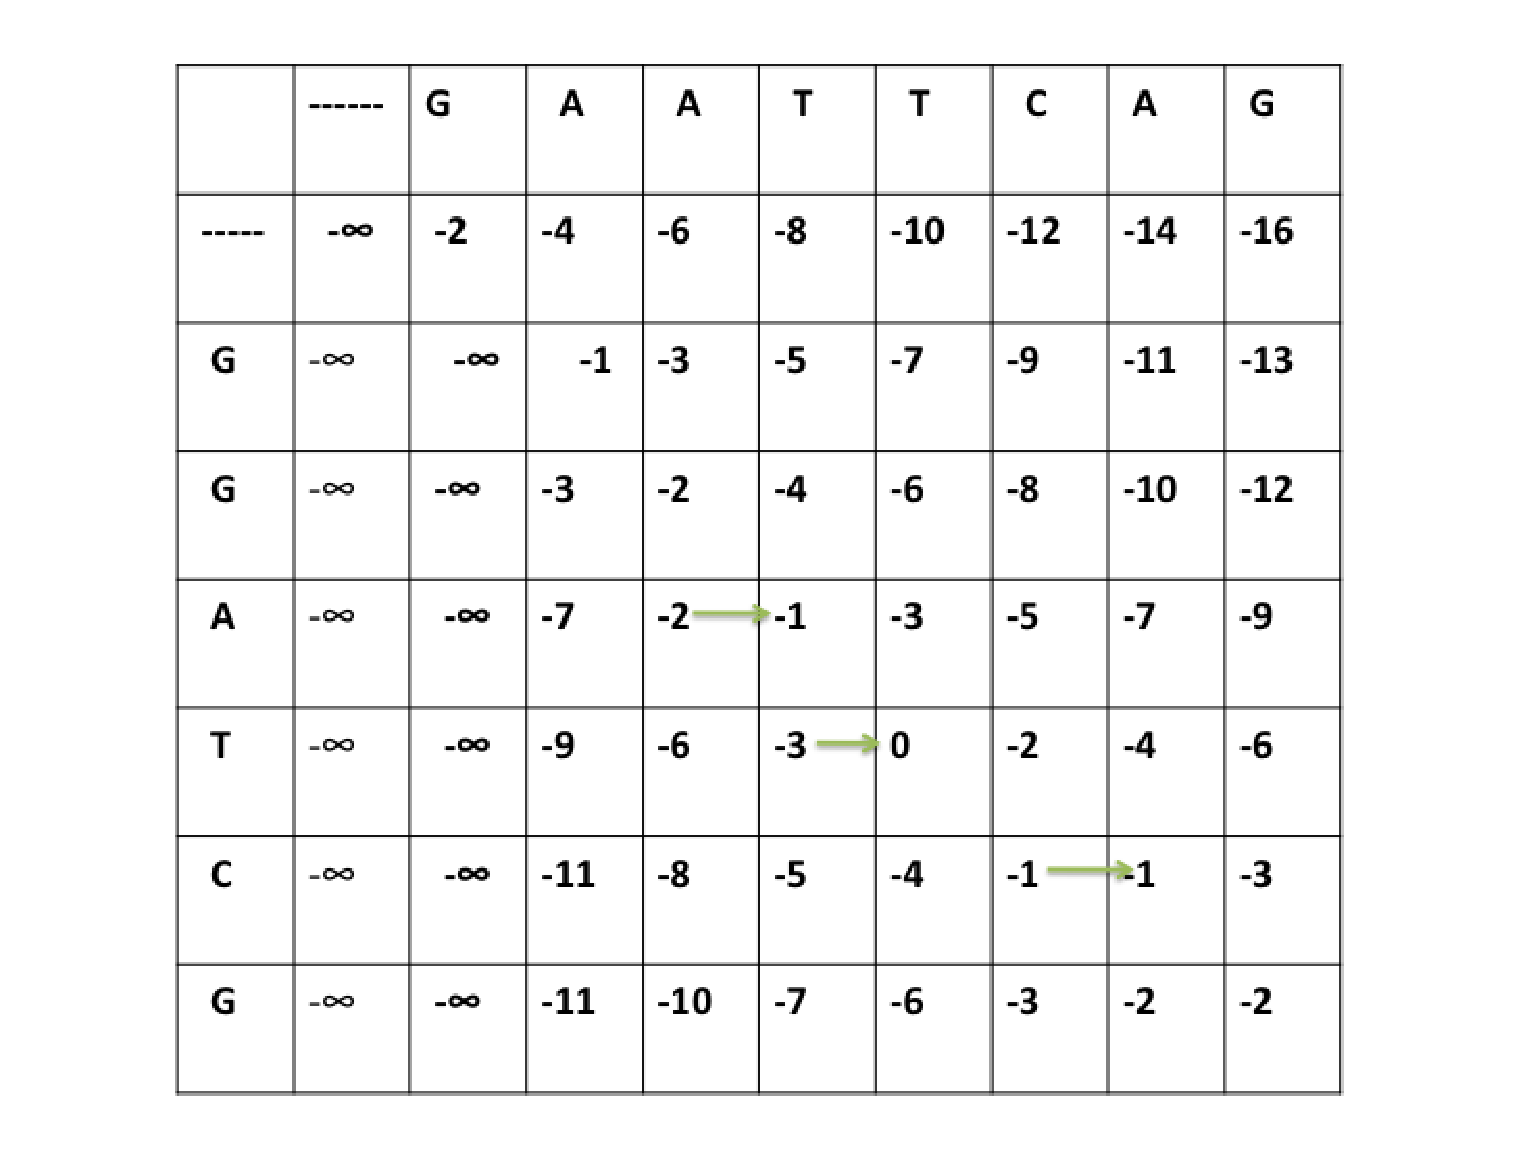
\includegraphics[width=4in]{Slide2}
\par\end{centering}

\caption{Matrix for deletion state}


%
\end{figure}


%
\begin{figure}
\begin{centering}
\caption{Matrix for insertion state}
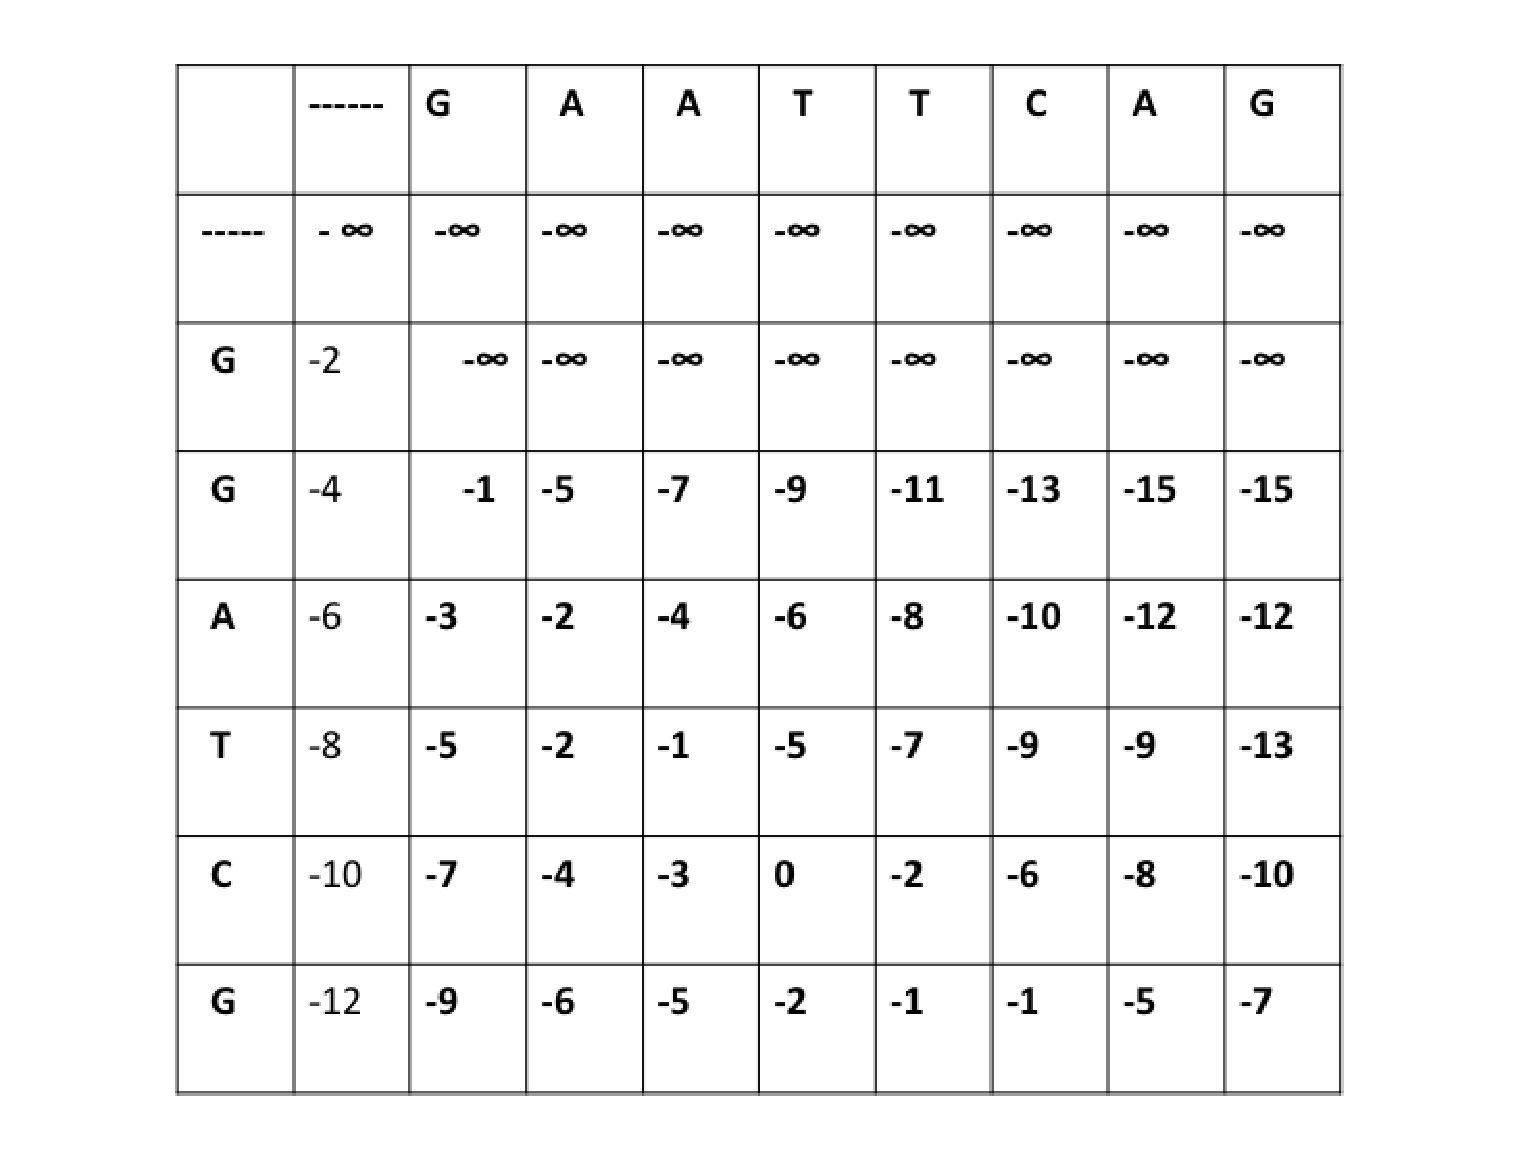
\includegraphics[width=4in]{Slide3}
\par\end{centering}

%
\end{figure}


%
\begin{figure}
\begin{centering}
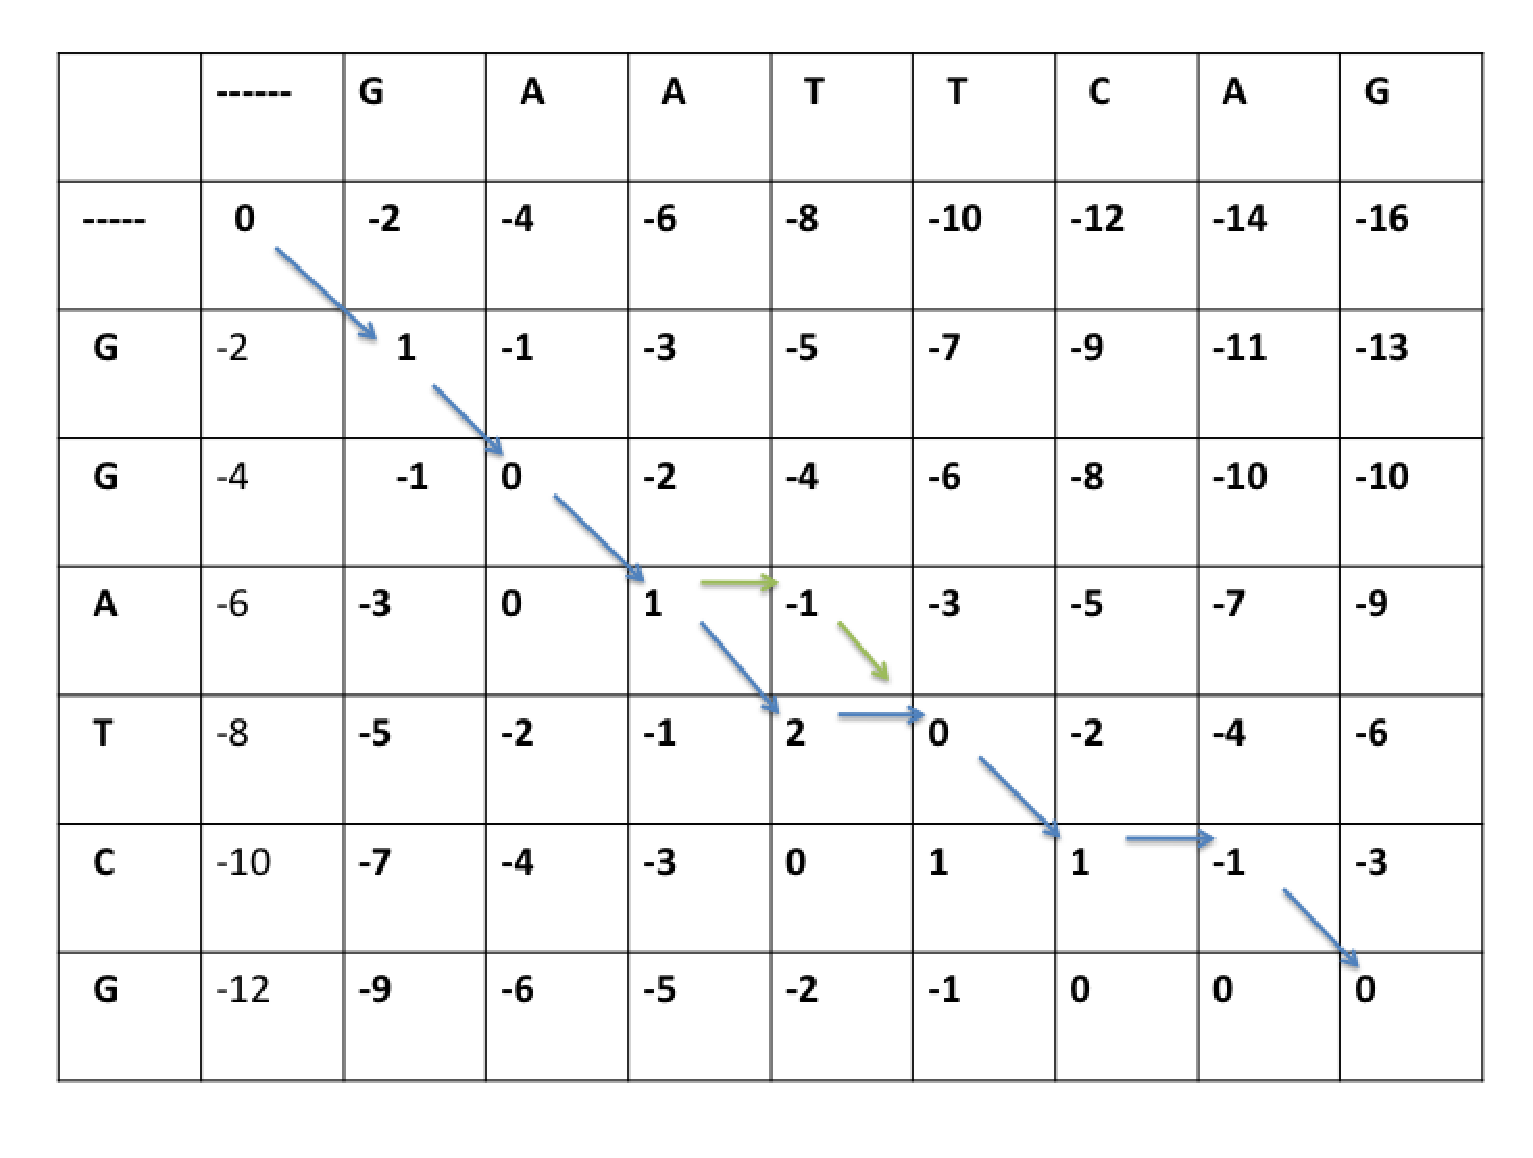
\includegraphics[width=4in]{Slide4}\caption{Alignment by backtracking}

\par\end{centering}

%
\end{figure}


There are two possible optimal alignments

%
\begin{figure}
\begin{centering}
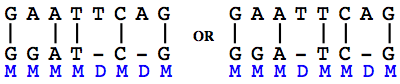
\includegraphics[width=2in]{alignment2}
\par\end{centering}

\caption{The alignments}


%
\end{figure}


\end{document}
